\section{Metodologia}
\label{sec:metodologia}

% ------------------------------- Apresentação Geral da Metodologia ------------------------------

Este trabalho adota uma abordagem metodológica estruturada em três fases para desenvolver uma interface gráfica intuitiva, estabelecer uma conexão robusta e validar o sistema em ambientes operacionais reais, com foco em robôs autônomos em ambientes internos e semi-estruturados. 

% --------------------------- Estratégia de Desenvolvimento e Validação --------------------------

A metodologia inicia com a análise do \textit{hardware} comercial disponível e a definição de requisitos técnicos. Em seguida, avança-se para o desenvolvimento paralelo dos subsistemas. Isso inclui a interface gráfica de usuário (GUI) com testes de usabilidade, a conexão robô-interface e os protocolos de comunicação via ROSBridge, conforme ilustrado na Figura \ref{fig:diagram}. O foco desta etapa é priorizar a exibição em tempo real de parâmetros essenciais, como posição, orientação e estado do sistema. Dessa forma, não são incorporados recursos avançados de aprendizado de máquina ou análise preditiva. A etapa final consiste em testes de integração e validação em ambientes simulados (RViz) e reais, limitados pelo período de desenvolvimento do trabalho acadêmico, o que restringe a quantidade de cenários avaliados.
% ---------------------- Abordagem Sequencial: Eficiência e Escalabilidade -----------------------

Essa abordagem sequencial assegura a verificação individual de cada componente antes da integração final, o que garante a eficiência operacional nas condições práticas previstas. Além disso, tal estrutura abre oportunidades para futuras expansões, como o desenvolvimento de componentes personalizados ou aplicações em ambientes externos.

\subsection{Análise do Hardware}
% -------------------------------- Caracterização do Hardware --------------------------------

A primeira fase da metodologia caracteriza o NVIDIA Jetson Orin Nano Developer Kit, plataforma do sistema robótico. O kit inclui um módulo Jetson Orin Nano 8GB com GPU NVIDIA Ampère (1024 núcleos CUDA), CPU de 6 núcleos e 8GB de memória LPDDR5, oferecendo até 40 TOPS (\textit{Tera Operations Per Second}) para aplicações de robótica. Sensores como LiDAR, IMU de 6 eixos e ultrassônicos, conectados via USB 3.2 Tipo-A ou conector de 40 pinos, suportam mapeamento 2D e navegação. Dois conectores MIPI CSI permitem câmeras para visão computacional. O armazenamento usa microSD ou SSD NVMe (M.2 Key-M). A comunicação ocorre via Wi-Fi, integrando com o ROS via ROSBridge \cite{NVIDIA_JetsonOrinNano}.


%Requisitos técnicos

%verificar 3D lidar ok

\subsection{Arquitetura do Sistema}

\begin{figure*}[htpb]
    \centering
    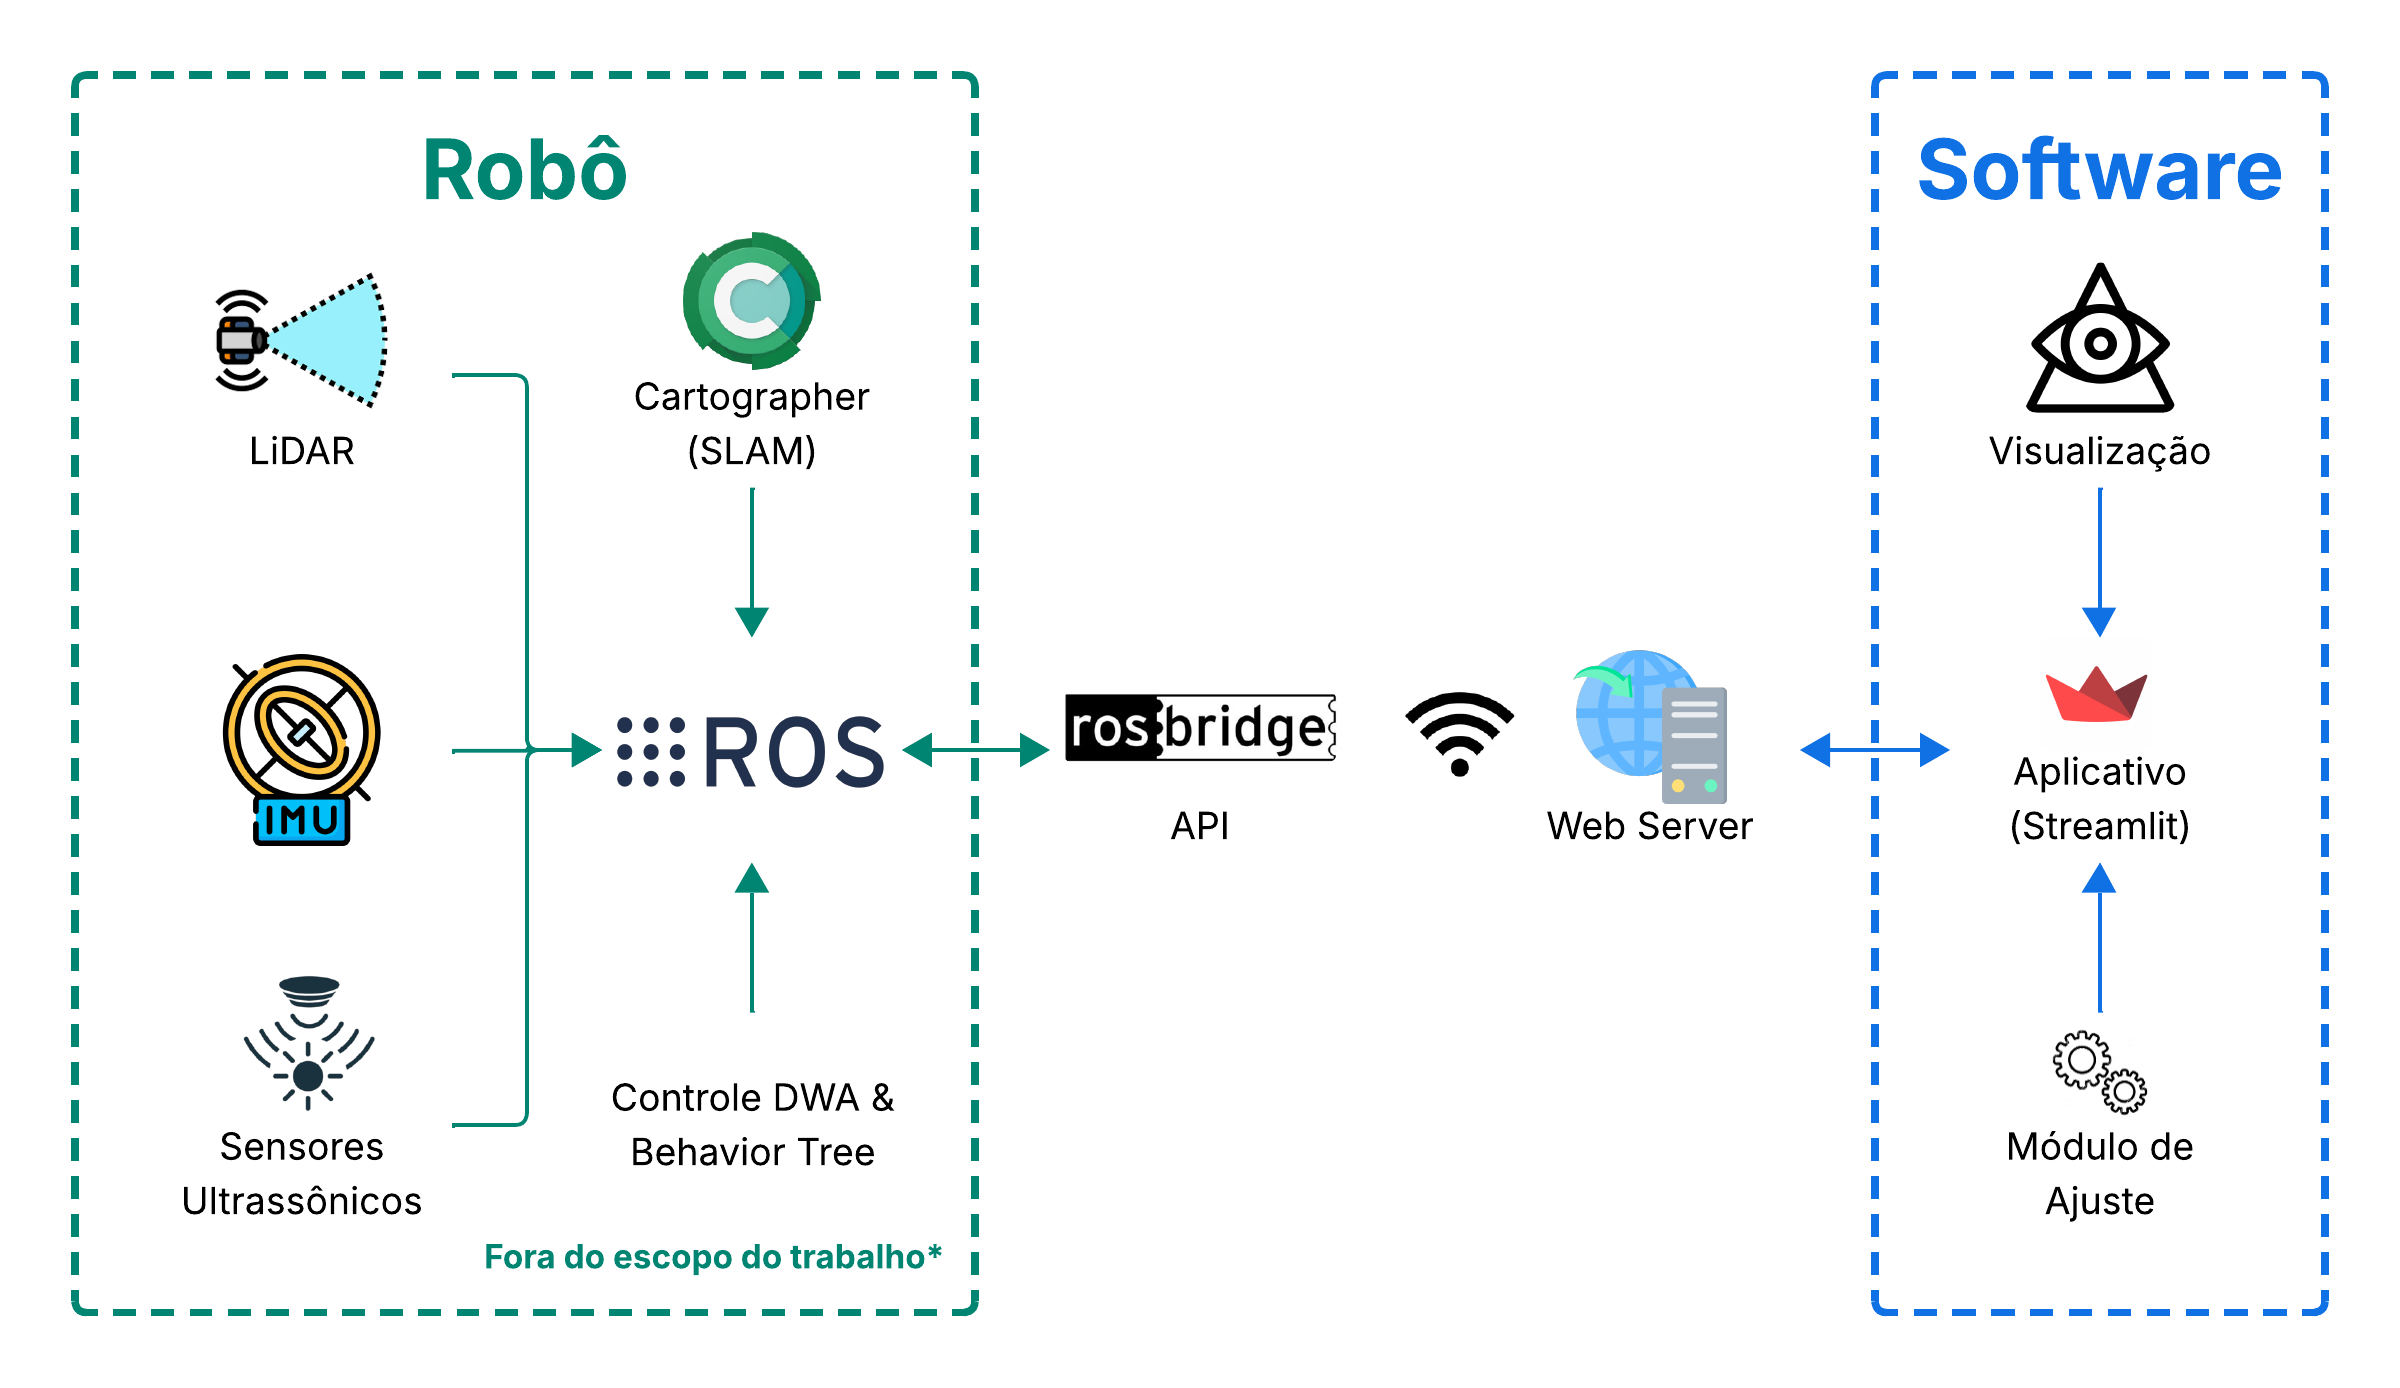
\includegraphics[width=\textwidth]{images/Diagrama_Arq.png}
    \caption{Diagrama da arquitetura do sistema.}
    \label{fig:diagram}
\end{figure*}

%fazer a chamada da figura no primeiro parágrafo. ok

O sistema robótico é projetado com uma arquitetura modular distribuída em três camadas principais, concebida para oferecer alta escalabilidade e flexibilidade na integração com diferentes plataformas robóticas e configurações de sensores. Na camada de percepção, os sensores atuam como os órgãos sensoriais do robô: um LiDAR para mapeamento 3D do ambiente, uma IMU de 6 eixos para medição inercial e sensores ultrassônicos para detecção de obstáculos próximos. 

A camada de processamento reside em um computador embarcado que opera o ROS (\textit{Robot Operating System}). Importante ressaltar que, apesar da nomenclatura, o ROS funciona como um \textit{framework} de software para robótica, e não como um sistema operacional em si. Essa camada estabelece a comunicação com os demais componentes através do ROSBridge, gerenciando a telemetria (incluindo dados de velocidade e status do sistema) e a integração direta com a interface. A ampla utilização do ROS como padrão na indústria e academia contribui para a facilidade de integração com uma diversidade de plataformas robóticas e dispositivos, o que intrinsecamente melhora a escalabilidade da arquitetura.

Na camada de interface com o usuário, o Streamlit \cite{Streamlit} fornece uma aplicação web acessível via navegador, exibindo dados de telemetria em tempo real e permitindo o controle manual quando necessário. A interface se conecta ao ROS através do ROSBridge, garantindo baixa latência na troca de comandos. Medidas de segurança como autenticação de usuário e criptografia serão implementadas para proteger a comunicação \cite{Streamlit}.

O fluxo de dados segue um ciclo contínuo: os sensores enviam informações para o ROS, que processa e toma decisões de navegação, enquanto a interface exibe os dados, recebe e envia comandos ao usuário. Os módulos são projetados para operar de forma independente em caso de falha pontual. A arquitetura desacoplada e a comunicação padronizada via ROS conferem ao sistema uma notável capacidade de adaptação e expansão, permitindo a integração com variados conjuntos de sensores e a fácil adição de novas funcionalidades.

% --------------------- Interface Gráfica ----------------------
%FAZER PROTÓTIPOS DE TELA E PENSAR NO FLUXO E USABILIDADE.
% VISUALIZAÇÃO PRÉVIA DE CADA MÓDULO
%CONTROLE
%VISUALIZAÇÃO DO MAPA - mapa, velocidade x, y, z, localização no mapa. Possibilidade de marcar pontos de passagem robo.
%Pensar como inserir lidar.
%CONFIGURAÇÃO/PARAMETRIZAÇÃO

%PARAMETRIZAÇÃO: velocidade mínima, velocidade máxima, modo teste, modo competição...

%https://balsamiq.com
O desenvolvimento da interface gráfica prioriza a criação de uma experiência intuitiva para o usuário final, com foco na implementação de um design responsivo que ofereça \textit{feedback} visual imediato para todas as interações. 

\begin{comment}
    
%não inserir nenhum parecer do que já foi feito na metodologia
A abordagem garantiu que a interface atendesse plenamente às necessidades de interação humano-robô, mantendo a simplicidade de uso sem comprometer a funcionalidade.
\end{comment}

% --------------------------- Comunicação ----------------------------

O módulo de comunicação é desenvolvido para garantir a troca de dados eficiente e confiável entre a interface e o robô. O protocolo ROSBridge é implementado para telemetria e integração com o sistema ROS, com atenção especial à redução de latência e manutenção da estabilidade da conexão.

%TROCAR TEMPO VERBAL DA METODOLOGIA - PRESENTE ok 

% ----------------------------- Tecnologias e Ferramentas Utilizadas -----------------------------

O sistema foi desenvolvido utilizando tecnologias complementares que atendem a cada componente específico. Para a interface, foi adotada a biblioteca Streamlit \cite{Streamlit}, que permite criar aplicativos web interativos com Python \cite{python3}, integrando-se diretamente ao núcleo do sistema ROS. Essa escolha elimina a necessidade de múltiplas linguagens e simplifica o desenvolvimento.

Também foram utilizadas outras duas bibliotecas Python: base64 para utilizar imagens no HTML e roslibpy\cite{ROSBridge} para comunicação da interface com o ROS.

A comunicação entre os módulos emprega o ROSBridge para telemetria geral e integração específica com o ROS. Essa combinação foi validada em trabalhos anteriores com requisitos semelhantes \cite{Teleoperacao}.

Para desenvolvimento e testes, o RViz\cite{rviz_wiki} está sendo utilizado para simulações iniciais e o Ceres Solver\cite{Ceres} para otimização numérica no mapeamento. A arquitetura resultante, apoiada por essas tecnologias validadas na literatura, oferece robustez operacional e facilidade de manutenção.

% -------------------------------- Requisitos da Interface --------------------------------

A interface gráfica para o sistema de telemetria e parametrização do robô autônomo é projetada com o objetivo de proporcionar uma interação intuitiva e eficiente entre o usuário e o robô, assegurando a visualização de dados em tempo real, a configuração de parâmetros operacionais e o controle manual, quando necessário. Com base na arquitetura modular e nas tecnologias empregadas, como o Streamlit e o protocolo ROSBridge, a interface é estruturada em dois módulos: Visualização e Controle. Esses módulos foram definidos para atender aos requisitos de usabilidade, alinhando-se aos objetivos do projeto e às demandas de interação humano-robô.

O módulo de visualização apresenta, em tempo real, informações essenciais como velocidade, posição e mapeamento do ambiente do robô. Esses dados são exibidos por meio de indicadores numéricos, com um mapa 2D gerado pelo algoritmo SLAM (Cartographer)\cite{Cartographer} para representar o terreno. Desenvolvida com Streamlit, a interface é responsiva, clara e acessível em dispositivos como navegadores web ou móveis, garantindo uma experiência amigável. A atualização dos dados ocorre com baixa latência, permitindo monitoramento contínuo.

O módulo de controle permite o usuário ajustar configurações operacionais, como limites de velocidade por meio de formulários interativos criados no Streamlit. Esses ajustes são enviados ao sistema via ROSBridge, garantindo uma comunicação rápida e segura. O módulo também oferece funcionalidades para operação manual utilizando setas direcionais para movimentação, essenciais em cenários que exigem intervenção humana, como testes ou situações de falha. A interface foi projetada para ser intuitiva, com elementos visuais que fornecem \textit{feedback} imediato, como confirmações de comandos. 

% ------------------------------ Critérios de Validação e Avaliação ------------------------------
\subsection{Critérios de Validação e Avaliação}

O sistema será avaliado em três aspectos principais: desempenho, robustez e usabilidade. 
 
% AVALIAR COMO SERÁ FEITO.

Os testes serão inicialmente realizados em ambiente simulado (RViz/ROS) para validação dos algoritmos e arquitetura. Após aprovação na simulação, o sistema será testado em condições reais, para verificar a robustez e a segurança da operação. Todos os resultados serão comparados com os requisitos técnicos estabelecidos.

% ------------------------------------- Limitações e Escopo --------------------------------------
\begin{comment}
%Mesclar esta informações no primeiro parágrafo da metodologia. De forma mais suave. ok


\subsection{Limitações e Escopo}

O presente trabalho foca no desenvolvimento de uma interface gráfica para telemetria e parametrização de robôs autônomos em ambientes internos e semi-estruturados, com algumas limitações definidas. Quanto ao escopo, não serão abordadas aplicações em ambientes externos ou condições climáticas adversas.

Quanto às limitações específicas da interface gráfica, o sistema está condicionado à visualização de dados provenientes exclusivamente dos sensores embarcados no robô, sem capacidade de fusão com fontes externas de informação ambiental. A arquitetura adotada prioriza a exibição de parâmetros essenciais para operação em tempo real, como posição, orientação e estado dos sistemas, em detrimento de visualizações 3D complexas ou reconstruções detalhadas do ambiente. A interface também não contempla recursos avançados de aprendizado de máquina para análise preditiva ou adaptação automática de layouts, mantendo-se focada em funcionalidades de telemetria e parametrização manual.

Em termos temporais, o projeto está limitado ao período de desenvolvimento do trabalho acadêmico, o que restringe a quantidade de cenários de teste que podem ser avaliados. Estruturalmente, a solução utiliza hardware comercial disponível, sem desenvolvimento de componentes eletrônicos customizados. Estas limitações, entretanto, abrem oportunidades claras para trabalhos futuros de expansão e aprimoramento do sistema.

\end{comment}